% !TEX root = ../main.tex

\chapter{全链路联合仿真}
\label{chap:joint}

\section{系统整合}

前述模型之间都隔着一个理想电源，后级负载无法影响前级。整机模型去掉 2200~V 理想电压源，把各环节放进同一个 Simscape 电气网络：10~kV 下垂调压电源经源阻抗和 10/1~kV 变压器接到双向平均值 AC/DC，直流母线接开关级 H 桥，H 桥驱动互感耦合的可变负载。退磁能量可以沿同一网络返回交流侧。

模型顶层如图~\ref{fig:int-model}(a) 所示，分为交直流供电、功率级、控制器、负载时序、时钟和观测六部分；供电子系统如图~\ref{fig:int-model}(b) 所示。表~\ref{tab:joint-map} 列出各环节的来源及整合时的处理。

\sidefig{native/model_int_system.png}{native/model_int_acdc.png}{整机模型（Simulink 原生视图）：(a) 顶层 \texttt{tokamak\_integrated}，(b) \texttt{ACDC\_Supply} 子系统}{fig:int-model}

\begin{dtable}{htbp}{已有模型到整机模型的映射}
\label{tab:joint-map}
\begin{tabularx}{\linewidth}{P{0.13\linewidth}P{0.36\linewidth}L}
\toprule
\headrow 来源 & 保留内容 & 整合处理 \\
\midrule
实验二 & 10~kV 电源、电网阻抗、无功下垂与电压 PI & 测试负载换成 10/1~kV 变压器和 AC/DC \\
实验三 & 四管 H 桥、单极性 PWM、2~kHz 载波、2~$\mu$s 死区 & 采用修正后的死区子系统，以 1~$\mu$s 求解 \\
实验四 & 电流 PI、互感回路、变参数时序、退磁控制 & 移除理想 2200~V 电源，接入实际母线 \\
新增 & 双向平均值 AC/DC，20~mF 直流缓冲电容 & 属于本项目的接口建模假设 \\
\bottomrule
\end{tabularx}
\end{dtable}

\section{双向平均值接口}

接口采用理想电网同步参考（频率 50~Hz，相位与电源相同），不模拟锁相环、整流器开关、滤波器和器件损耗。令 $\theta=2\pi\times50t$，变比 $r=2200/1000=2.2$，开关函数向量为
\begin{equation}
\boldsymbol m=r\sqrt{\tfrac23}\begin{bmatrix}\sin\theta&\sin(\theta-\tfrac{2\pi}{3})&\sin(\theta+\tfrac{2\pi}{3})\end{bmatrix}^{\mathrm T}.
\end{equation}
端口关系为
\begin{equation}
V\sub{dc}=\boldsymbol m^{\mathrm T}\boldsymbol v\sub{abc},\qquad \boldsymbol i\sub{ac}=-\boldsymbol m\,i\sub{dc},
\label{eq:acdc}
\end{equation}
其中 $i\sub{dc}$ 以流入变换器直流正端为正，于是每一时刻都有 $\boldsymbol v\sub{abc}^{\mathrm T}\boldsymbol i\sub{ac}+V\sub{dc}i\sub{dc}=0$：功率可以双向传递，接口自身不储能。对与参考同相的平衡正弦电压，$V\sub{dc}=rV\sub{LL,rms}$。

这是理想变换级的聚合关系，变比并不代表某个已设计好的两电平整流器能够实现该增益。20~mF 缓冲电容预充至 2200~V（初始储能 48.4~kJ）。2200~V 是接口额定点，实际母线电压随交流侧变化；电流环仍按名义 2200~V 换算调制比，没有增加直流母线外环。

全局求解器为固定步长 ode3，步长 1~$\mu$s，Simscape 局部后向欧拉每步 3 次非线性迭代；30~s 工况实际耗时约 16~min。死区判断先映射回 1~$\mu$s 时钟格点（第 \ref{chap:hb} 章）。综合信号每 10~$\mu$s 记录一次，能量在模型内部按 1~$\mu$s 积分，报告中的能量都取自这些积分通道。

\section{全程运行结果}

整机从零时刻连续运行到 30~s，覆盖升流、平台、降流与退磁（图~\ref{fig:int-wave}），平台段统计见表~\ref{tab:int-platform}。$i\sub{p}$ 均值 9999.28~A，跟踪给定 10~kA；全程结束时线圈电流约 $-4.2\times10^{-8}$~A，磁链回到零。母线全程在 2187.0--2219.2~V 之间，只偏离额定点约 $\pm1\%$，峰值出现在 12.3~s 切入退磁的瞬间。

\twofig{native/int_currents_dc.pdf}{native/int_power_energy.pdf}{整机 30~s 运行的 MATLAB 原生波形：(a) 等离子体电流、线圈电流和母线电压，(b) 各级功率与净能量}{fig:int-wave}

\begin{dtable}{htbp}{整机运行的平台段统计（6--11~s）}
\label{tab:int-platform}
\begin{tabularx}{\linewidth}{P{0.26\linewidth}RP{0.26\linewidth}R}
\toprule
\headrow 指标 & 数值 & 指标 & 数值 \\
\midrule
母线电压平均值 & 2199.98~V & 交流侧有功 & 1.1259~MW \\
母线电压最小 / 最大 & 2199.08 / 2200.83~V & 交流侧无功 & $-0.012$~Mvar \\
等离子体平均电流 & 9999.28~A & 线圈侧功率 & 1.0781~MW \\
原边平均电流 & 10\,749.17~A & 交流母线电压 & 1.00005~pu \\
直流侧电流平均值 & 512.2~A & 内部电势 & 1.0022~pu \\
\bottomrule
\end{tabularx}
\end{dtable}

交流母线电压 1.00005~pu，与由 $Q=-0.012$~Mvar 计算的下垂目标 1.00006~pu 一致；无功接近零，因此下垂几乎不动作，内部电势只需抬高 0.22\% 以补偿有功电流的阻抗压降（图~\ref{fig:int-grid}(a)）。接口是平均值模型且假设同步，这个结果不能理解为全工况单位功率因数，负载造成端口电压相移时无功并不严格为零。

\section{能量闭合与退磁回馈}

理想接口使交流侧与直流侧的累计能量完全相等，功率残差不超过 $10^{-9}$ W，缓冲电容净储能变化可以忽略。全程净能量：交流侧与直流侧 11.1059~MJ，线圈侧 10.5964~MJ，差值 0.5095~MJ 是 H 桥器件损耗。

\twofig{native/int_grid_response.pdf}{native/int_demag_return.pdf}{MATLAB 原生波形：(a) 交流侧电压、功率与负载时序，(b) 退磁段的电流、功率和自 12.3~s 起的净能量}{fig:int-grid}

退磁段的能量逐级可以对上（图~\ref{fig:int-grid}(b)）。互感磁场储能峰值 $\tfrac12L_1i\sub{m}^2=0.588$~MJ；12.3--30~s 线圈向 H 桥净回馈 0.565~MJ，向交流侧净回馈 0.559~MJ，逐级减少的部分对应 $R\sub{cs}$ 和器件损耗。

\section{门极、纹波与数值检查}

启动（1.98--2~s）和末段（29.98--30~s）两个 1~$\mu$s 门极窗口都测得 2~$\mu$s 死区，桥臂重叠导通的记录数为 0（图~\ref{fig:int-gate}(b)）。平台段电流纹波峰峰值 226.55~A，母线上对应约 $\pm3$~V 的开关纹波（图~\ref{fig:int-gate}(a)）。

启动工况把每步非线性迭代由 3 次增加到 6 次，两路电流的最大绝对差约 $1.45\times10^{-8}$~A。这只是该工况的数值敏感性检查，并不构成全工况的收敛证明。四个基线模型在布局整理前后做了逐点比较，保存的信号和 Simscape 日志完全一致，这一结论只针对基线的布局整理，不适用于改变了功能的修正版和整机模型。

\twofig{native/int_current_dc_ripple.pdf}{native/int_deadtime_zoom.pdf}{MATLAB 原生波形：(a) 1.8--1.82~s 的等离子体电流和母线电压纹波，(b) 两桥臂换相的 2~$\mu$s 死区}{fig:int-gate}

\section{晶闸管整流接口的对照}

项目同时保留了另一套联合模型（分支 \texttt{task05-system-integration}），接口采用真实的六晶闸管全控桥：10/1.2~kV 变压器、5~mH 平波电抗器、0.2~F 母线电容，目标电压 1500~V，功率级步长 2~$\mu$s。桥只能单向供能，退磁能量无法回到电网，因此增设滞环制动支路：母线达到 1650~V 时投入 5~$\Omega$ 电阻，降到 1600~V 时退出。

这一接口带来了平均值模型中没有的问题。空电容直接充电时母线峰值约 2.58~kV，为此把电压参考改为 0--0.5~s 线性上升，并引入 0.01 $^\circ$/A 的电流阻尼（图~\ref{fig:thy}(a)）。退磁回馈约 0.56~MJ，电容从 1500~V 升到 1650~V 只能吸收 47.25~kJ，其余由制动电阻消耗（图~\ref{fig:thy}(b)）。降流开始后 H 桥不再取用功率，电压环把触发角推到 $85^\circ$ 上限，整流器基本停止输出（图~\ref{fig:thy}(c)）。平台段平均触发角 19.42$^\circ$，低于式~\eqref{eq:rect} 的 22.19$^\circ$，多出的电压裕量用于补偿 0.02~$\Omega$ 电阻、晶闸管压降和换相压降；一次侧电流呈现六脉波的典型畸变（图~\ref{fig:thy}(d)）。

\begin{figure}[htbp]
\centering
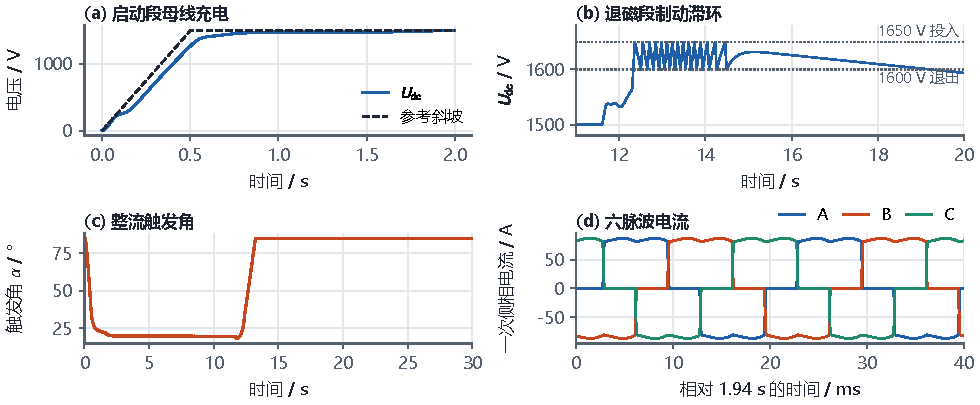
\includegraphics[width=\linewidth]{thyristor_interface}
\caption{晶闸管接口联合模型的运行结果（由保存的数据绘制）}
\label{fig:thy}
\end{figure}

该模型的全程能量流向见图~\ref{fig:joint-sankey}。按直流侧功率平衡方程核算，整流输出减去 H 桥输入、制动、泄放和电容储能变化后，全程残差 0.3797~kJ，相对整流输出为 0.00318\%。800 次换相的死区均为 2~$\mu$s，无同臂同时导通。步长由 2~$\mu$s 减为 1~$\mu$s 时，1.96--2~s 窗口的平均母线电压相差 0.017~V，平均电流相差 0.060~A，纹波由 251.21~A 降到 225.81~A。

\begin{figure}[htbp]
\centering
\begin{tikzpicture}[font=\footnotesize, >={Latex[length=1.6mm]},
  stage/.style={draw=#1, fill=#1!8, rounded corners=1.5pt, line width=0.6pt, align=center, minimum width=21mm, minimum height=12mm, inner sep=1pt},
  flow/.style={->, line width=0.8pt, color=black!70},
  sink/.style={draw=black!45, fill=rowtint, rounded corners=1.5pt, line width=0.5pt, align=center, minimum width=21mm, minimum height=8mm, font=\scriptsize, inner sep=1pt},
  drop/.style={->, line width=0.5pt, color=black!50}]
\node[stage=segbus] (g) at (0,0) {10~kV 母线送出\\\textbf{12.077~MJ}};
\node[stage=segrect] (r) at (3.2,0) {整流直流输出\\\textbf{11.936~MJ}};
\node[stage=seghb] (h) at (6.4,0) {H 桥直流输入\\\textbf{11.103~MJ}};
\node[stage=segpl] (c) at (9.6,0) {线圈侧输入\\\textbf{10.595~MJ}};
\node[stage=segpl] (p) at (12.8,0) {等离子体电阻\\\textbf{10.559~MJ}};
\draw[flow] (g)--(r);
\draw[flow] (r)--(h);
\draw[flow] (h)--(c);
\draw[flow] (c)--(p);
\node[sink] (a) at (0,-1.7) {变压器与桥损耗等\\0.141~MJ};
\node[sink] (b) at (3.2,-1.7) {制动 0.531~MJ\\泄放 0.071~MJ\\电容增量 0.230~MJ};
\node[sink] (d) at (6.4,-1.7) {H 桥器件损耗等\\0.508~MJ};
\node[sink] (e) at (9.6,-1.7) {$R\sub{cs}$ 等\\0.036~MJ};
\draw[drop] ($(g.east)+(0.25,0)$) |- (a.east);
\draw[drop] ($(r.east)+(0.25,0)$) |- (b.east);
\draw[drop] ($(h.east)+(0.25,0)$) |- (d.east);
\draw[drop] ($(c.east)+(0.25,0)$) |- (e.east);
\end{tikzpicture}
\caption{晶闸管接口模型 30~s 全程的能量流向。H 桥与线圈侧为代数累计，已扣除退磁回馈}
\label{fig:joint-sankey}
\end{figure}

两套模型由不同组员独立搭建，接口和母线电压都不相同，负载侧结果却高度一致（表~\ref{tab:compare}）：线圈侧能量相差 0.015\%，H 桥直流输入能量相差 0.03\%，1~$\mu$s 下的纹波相差 0.3\%。这说明负载和 H 桥的行为基本不受前级接口影响。差别集中在前级：晶闸管接口的交流侧送出能量多约 0.97~MJ，主要是制动消耗、母线电容留存和整流损耗，而双向接口把这部分回馈给了交流侧。

\begin{dtable}{htbp}{两种联合模型的对照}
\label{tab:compare}
\begin{tabularx}{\linewidth}{LRR}
\toprule
\headrow 项目 & 双向平均值接口 & 晶闸管整流接口 \\
\midrule
变压器与母线额定 & 10/1~kV，2200~V & 10/1.2~kV，1500~V \\
母线电容 & 20~mF & 0.2~F \\
退磁能量去向 & 回馈交流侧 & 电容与制动电阻 \\
母线电压范围 & 2187.0--2219.2~V & 最高 1650.14~V \\
功率级步长 & 1~$\mu$s & 2~$\mu$s（对比 1~$\mu$s） \\
平台段原边电流 & 10\,749.17~A & 10\,749.42~A \\
1~$\mu$s 电流纹波峰峰值 & 226.55~A & 225.81~A \\
交流侧累计能量 & 11.1059~MJ & 12.0770~MJ \\
H 桥直流输入累计能量 & 11.1059~MJ & 11.1030~MJ \\
线圈侧累计能量 & 10.5964~MJ & 10.5948~MJ \\
\bottomrule
\end{tabularx}
\end{dtable}
